%	Copyright (C) 2008, 2009 Julian M. Kunkel
%
%	This file is part of PIOsimHD.
%
%	PIOsimHD is free software: you can redistribute it and/or modify
%	it under the terms of the GNU General Public License as published by
%	the Free Software Foundation, either version 3 of the License, or
%	(at your option) any later version.
%
%	PIOsimHD is distributed in the hope that it will be useful,
%	but WITHOUT ANY WARRANTY; without even the implied warranty of
%	MERCHANTABILITY or FITNESS FOR A PARTICULAR PURPOSE.  See the
%	GNU General Public License for more details.
%
%	You should have received a copy of the GNU General Public License
%	along with PIOsimHD.  If not, see <http:%www.gnu.org/licenses/>.


\documentclass[
     11pt,         % font size
     a4paper,      % paper format
     BCOR10mm,     % binding correction
     DIV14,        % stripe size for margin calculation
     liststotoc,   % table listing in toc
     bibtotoc,     % bibliography in toc
     idxtotoc,     % index in toc
     parskip       % paragraph skip instad of paragraph indent
     ]{scrreprt}   %report
\usepackage{times}

\usepackage[numbers]{natbib}

%\font\klingon=klinz

\citeindextrue

%%%%%%%
\usepackage[left=2.1cm,top=1.8cm,right=2.1cm,bottom=2.4cm]{geometry}
\usepackage{courier}

\usepackage[USenglish]{babel}
% Input encoding
\usepackage[utf8]{inputenc} 
% Font encoding
\usepackage[T1]{fontenc}
% Index-generation
%\usepackage{makeidx}
% Einbinden von URLs:
\usepackage{url}
% Special \LaTex symbols (e.g. \BibTeX):
\usepackage{doc}
% Include Graphic-files:
\usepackage{graphicx}
\usepackage{amsmath}
% Include doc++ generated tex-files:
%\usepackage{docxx}
% Include PDF links
\usepackage[pdftex, bookmarks=true]{hyperref}
\usepackage{enumitem}
\usepackage{fancybox}
\usepackage{rotating}
\usepackage{subfigure}
%%%%%%%%%%%%%%%%%%%%%%%%%%%%%%%%%%%%%%%%%%%%%%%%%%%%%%%%%%%%


% OTHER SETTINGS:
%\usepackage[pdftex,colorlinks,linkcolor=blue]{hyperref}
\newcommand{\myTitle}[0]{
Simulation of Parallel I/O and MPI Communication with a Discrete Event Simulator
}

\newcommand{\cmd}[1]{\texttt{#1()}}

\newcommand{\fatRot}[1]{
  \begin{turn}{-90}
   \textbf{#1}
  \end{turn}
 }

\usepackage{color}
\usepackage{listings} \lstset{numbers=left, numberstyle=\tiny, numbersep=5pt}
\lstset{language=Java} 
\lstset{frame=shadowbox, numbers=none,  rulesepcolor=\color{black}}
%\lstset{basicstyle=\ttfamily\scriptsize}
\lstset{ showspaces=false}

% Pagestyle:
\pagestyle{headings}

% Choose language
\newcommand{\setlang}[1]{\selectlanguage{#1}\nonfrenchspacing}

\newcommand{\includescalepngs}[1]{
\includegraphics[scale=0.5]{../bilder/#1}
}

\newcommand{\client}{ \begin{enumerate}[label=C\arabic{*}, ref=C(\arabic{*})]  }


\hypersetup{
	pdftitle = {\myTitle},
	pdfsubject = {Technical Report},
	pdfauthor = {Julian Martin Kunkel},
	pdfkeywords = {Parallel File Systems, High Performance Computing, MPI, Simulation}
}

\begin{document}
\begin{titlepage}

\vspace*{1cm}
\begin{center}
\textbf{
\Large Ruprecht-Karls-Universität Heidelberg\\
\smallskip
\Large Institut für Informatik\\
\smallskip
\Large Arbeitsgruppe Parallele und Verteilte Systeme\\
\smallskip
}

\vspace{3cm}

\textbf{\large Technical Report} 

\vspace{0.5\baselineskip}
{\huge
\myTitle
}
\end{center}

\vfill

{\large
\begin{tabular}[l]{ll}
Julian Martin Kunkel\\
January 2009
\end{tabular}
}

\end{titlepage}

\tableofcontents

\chapter{Introduction}
\section{Clusters}
* Cluster, Nodes, Bottleneck

\section{Message Passing Interface}
** Communication

\section{Parallel file systems}
** Optimizations, ROMIO


\section{Goals}
\begin{itemize}
\item Fast prototyping of new algorithms, for I/O optimization and MPI
\item Reveal bottlenecks.
\item Teaching, better understanding of observed system behavior
\item Test applications on different cluster hardware i.e. GRIDs
\item Simple but extendible models which can be selected on demand.
   Explicit abstraction from the real world complexity (for instance TCP Sliding Windows algorithm).
   However, similar results (runtime) to real world experiments should be possible
\item Usage of common tools to analyze simulation results.
\item Real OpenSource Software
\end{itemize}

\section{State of the Art}
\subsection{Simulators}
** Paraver / Dimemas
** Starfish
** The Network Simulator
** GTNets
** NCTUns 4.0

%* Performance optimization
%** ROMIO: Two-Phase-I/O, 

\subsection{Models}
Realistic Communication Model for Parallel Computing on Cluster.
http://i.cs.hku.hk/~clwang/papers/model-iwcc99.ps



\chapter{Model}

\begin{figure}[!htbp]
  \centering
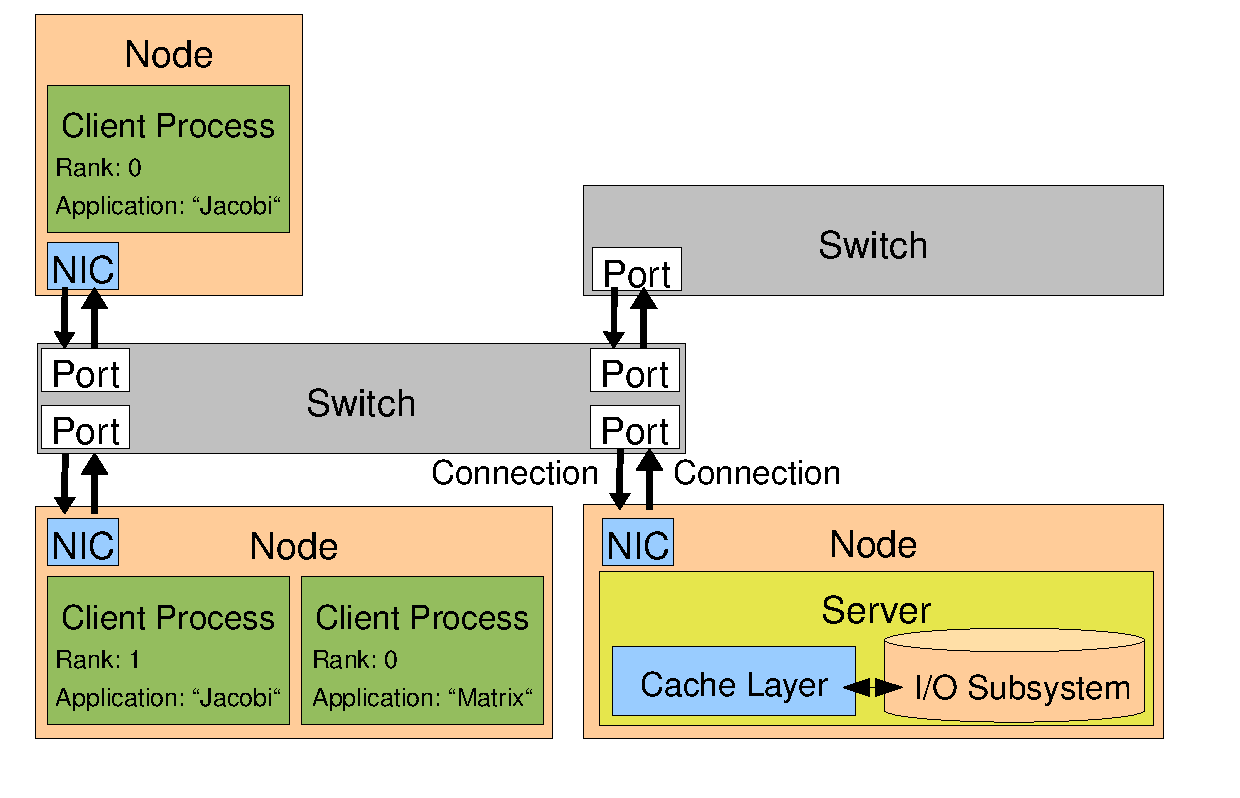
\includegraphics[scale=0.5]{Images/cluster-model.pdf}
    \caption{Example cluster component model}
    \label{fig:cluster-model}
\end{figure}

\begin{figure}[!htbp]
  \centering
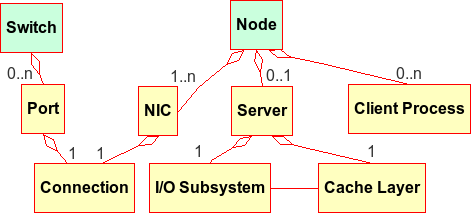
\includegraphics[scale=0.5]{Images/cluster-components.png}
    \caption{UML diagram showing the relations between cluster components}
    \label{fig:cluster-relation}
\end{figure}


* Exchangable component behavior
  Interfaces are not completely specified and can be modified as required.

\section{Elementary Components}
\subsection{Node}
\subsection{Network Interface Card (NIC)}
\subsection{Client Process}
\subsection{Server Process}
\subsection{Server Cache Layer}
\subsection{I/O Subsystem}
\subsection{Switch}
\subsection{Port}
\subsection{Connection}

\section{Application}
\subsection{Program}
\subsection{Command}

\section{Logical Files}



\chapter{PIOsimHD Package}
\section{Source Code}
* Split into Model, GUI, Simulation
\section{Provided Binaries/Scripts} %Example Usage
piosimhd
tau2slog2
jumpshot




\chapter{Design}

\section{Design Principles}
* Reflection
* Annotations
* Basic Model Classes contain Data
* Generation of Model, on run-time the simulator instanciates classes depending on the user configuration implementing such a model. The model is fixed during simulation.

\section{Model Generation}
* A model can be stored explicitly in XML or implicit in Java code.
Builder classes assist to build a (normal) model on the fly.
See the code example in \ref{lst:exampleClusterBuild}. 
A GUI is planned to easy generation of a cluster model for teaching.


\section{XML Generation}
* serialization of annotated attributes

\section{Command Execution}
MPI-Commands are executed as statemachines, for each type of commands (e.g. broadcast operations) one class instance is loaded and responsible to run commands on all clients. 
Therefore, the class instance knows the status of all client operations of the same type.
The processing of a operation is encoded in the method process of the particular class:
\begin{verbatim} 
	public void process(Bcast cmd, CommandProcessing OUTresults, GClientProcess client, int step, NetworkJobs compNetJobs)
\end{verbatim}
Arguments to the command (for example communicator in broadcast or data size) is contained in \texttt{cmd}.
The result of process must be stored in \texttt{OUTresults}.
Upon initial startup of a command the \texttt{step} number is \texttt{CommandProcessing.STEP_START}.

An operation can access answers of other clients in the \texttt{compNetJobs} datastructure.

A command can decide to invoke other commands to process a command,
assume a dynamic broadcast, which chooses existing MPI implementations for a broadcast, based on the given parameters.
\begin{verbatim}
 OUTresults.invokeChildOperation(cmd, CommandProcessing.STEP_COMPLETED, de.hd.pvs.piosim.simulator.program.Bcast.BinaryTreeSimple.class);
\end{verbatim}

To communicate with other processes, messages can be either sent or received to another process number of the
given communicator:
\begin{verbatim}
OUTresults.addNetSend(1, new NetworkSimpleData(20), // just 20 Bytes or something.
  30002, Communicator.INTERNAL_MPI);
\end{verbatim}
The tag and communicator on sender and receiver side must match, then the receiver gets the message.

The statemachine will not proceed to the next step until all messages of one step are sent and received.

Therefore, to create a parallel pipeline to multiple clients it is required to create a pipelined point to point connection,
then for each participating host spawn one pipelined child operation. 
Now all pipelines could process concurrently.

\section{Choosing Component and Command Implementations}
The component and command implementations can be chosen dynamically.

Command mapping is stored explicitly in the XML file.
Available commands and the mapping from a particular modeled command to available
implementations is encoded in a simple text file.
An excerpt of the mapping is given in listing \ref{lst:commandMapping}.
For each command the implementation used during a simulation must be specified and is used across
all client processes. Imagine to combine a dummy MPI\_Barrier implementation which
does not send any message with another implementation sending messages for synchronization.
Obviously this will not work. Due to the reason that it does not make sense to pick different
implementations for a command on different processes only one implementation can be chosen for
a particular command.
If the implementation is not specified in the model XML file by default the last implementation 
in the text file is chosen

\begin{lstlisting}[numbers=none,caption=CommandToSimulationMapper.txt,label=lst:commandMapping,language=Perl,basicstyle=\ttfamily\scriptsize]
# define the command groups and the contained implementations and the simulator
# implementations each row is either a set of commands which are implemented or
# the actual set of implementation classes for these commands.
# In the following ... abbreviates de.hd.... prefix, just for visualization!

+de.hd.pvs.piosim.model.program.commands.Compute
de.hd.pvs.piosim.simulator.component.Commands.Global.Dummy
de.hd.pvs.piosim.simulator.component.Commands.Compute.Time

#define a group of commands which belong together:
+de.hd.pvs.piosim.model.program.commands.Send,...commands.Receive,...commands.Sendrecv
de.hd.pvs.piosim.simulator.component.Commands.Global.Dummy...Dummy,...Dummy
...SendReceive.Rendezvous.RendezvousSend,....RendezvousRcv,...RendezvousSendrecv

...
\end{lstlisting}

In the cluster model each particular component can have its own model class.
For instance one I/O server can use a different disk model from a second server. (In this example
assume a RAID disk and a flash drive).
For each model class one simulation class can be choosen in a text file. The implementation class
uses the data provided in the model class to simulate the behavior.
An excerpt of the mapping is given in listing \ref{lst:modelMapping}.

\begin{lstlisting}[numbers=none,caption=ModelToSimulationMapper.txt,label=lst:modelMapping,language=Perl,basicstyle=\ttfamily\scriptsize]
# This file describes the existing model component of a given type e.g. "Node"
# the available Model implementations and mapping to the simulation implementation.
# Syntax <Model Implementation> = <Simulation Implementation>

+ClientProcess
de.hd.pvs.piosim.model.components.ClientProcess.ClientProcess =
  de.hd.pvs.piosim.simulator.component.ClientProcess.GClientProcess

+IOSubsystem
de.hd.pvs.piosim.model.components.IOSubsystem.SimpleFlash =
  de.hd.pvs.piosim.simulator.component.IOSubsystem.GSimpleFlash
de.hd.pvs.piosim.model.components.IOSubsystem.SimpleDisk =
  de.hd.pvs.piosim.simulator.component.IOSubsystem.GSimpleDisk
de.hd.pvs.piosim.model.components.IOSubsystem.RefinedDiskModel =
  de.hd.pvs.piosim.simulator.component.IOSubsystem.GRefinedDiskModel

...
\end{lstlisting}

\subsection{Data Flow}
There are two aspects, one is how pakets are transported within the network, second handles internal processing of requests on simulated I/O servers.

\subsubsection{Network packet transport}
Design criteria: 
\begin{itemize}
 \item (almost) optimal network usage - it is mandatory that network components can be fully utilized if there are packets to transport.
 \item realistic transport - data flows must look somehow realistic, if there is a bottleneck it is not acceptable that all packets queue on this component. 
  In reality in switched networks buffers allow a limited queue, retransmits occur on packet loss, timeouts on NICs resent lost packets. 
  However, especially timeouts are hard to estimate, any delay can lead to idle times on the network.
  Wormhole routing on the other hand may reserve bandwidth, but if the packets are delayed reserved bandwidth is wasted.   
 \item Simplicity - to some extend observed behavior should be understandable.
 \item Performance of the implementation - the implementation should not heavily impact simulation performance.
\end{itemize}

Several alternatives have been tested, for example timeout based retransmit with limited cache size.
However, the current design models flow control as follows:
\begin{itemize}
 \item A network component transmits a number of packets to another until more data got send to compensate for connection  latency. 
 Then the component stalls submission and queues further packets. 
 \item Processing of a packet confirms the receipt to the sender and allows to transfer packets worth for the connection latency compensated by the accepted packet. 
 Therefore, processing of a packet might wake up a cascade of blocked components upstream.
 \item Once a component finishes processing of a packet it shall accept new packets. Pending packets should be delivered immediately to avoid starvation of downstream components.
 \item On each component packets are queued per target in the network. 
  Depending on the receiver in the network a separate queue exists.
  If one queue is stalled then another queue might still proceed. 
  To understand the reason, assume a complex topology in which network components are interconnected with varying speeds. 
  In this scenario one slow target might lead to queues in the intermediate switches. 
  However, other network components with fast interconnects must still get their performance, therefore the switches must allow to relay their packets. 
 \item NICs must allow block receiving of further packets. 
  This is necessary for example on I/O processes. 
  Writing data to a file system ships data to I/O processes. If the I/O subsystem controlled by this process is slower than the network card, then data is (potentially infinitely) queued on the I/O process. 
  This is not realistic, therefore the process must block transmission once it has no more free RAM to accept data.
  \item Packet size is limited by a \textbf{NetworkGranularity} to ensure interleaved processing of packets. 
  Messages are partitioned into the NetworkGranularity on demand. 
  Two aspects are involed into picking the size, smaller packets result in more events in the simulation i.e. increase simulation time, but allow a better interleaving of packets from multiple sources on one network component.   
  Bigger packets decrease simulation efford but reduce interleaving. 
\end{itemize}

\subsubsection{I/O Server request processing}
From client side an I/O request is just issued with an list of offset and size pairs (list-IO).
These lists of non-contiguous operations could be generated automatically by file views.

Once the client issues an I/O operation, the actual visible operation consists of several steps, which are processed sequencially.
An I/O involves client, server process including cache layer of data and I/O subsystem, network cards and intermediate network. 
Data flow through the network is already discussed, consequently it is spared here.
Processing of I/O requests depends on the actual request type i.e. read or write.

\paragraph{Read request}
\begin{itemize}
 \item client submits an read request to the NIC
 \item network transmits requests to all servers involved in the I/O
 \item each server accepts the request and announces the complete request to its cache layer
 \item cache layer selects an I/O operation to work on and submits this operation to the I/O subsystem (the I/O subystem model might allow queue up multiple operations). Note the size of a single contiguous I/O operation is limited to \textbf{IOGranularity}.
 \item once the I/O subsystem finished an operation the cache layer is notified and might submit new operations. 
 Also data received from the cache layer is immediately added to the network flow resulting in new packets for the network.
 \item client I/O is implicitly finished once all data is received
\end{itemize}

\paragraph{Write request}
\begin{itemize}
 \item client submits a write request to all servers involved in the I/O
 \item each server accepts the request and responds with an acknowledge
 \item client waits for all acknowledges and starts I/O stream to all servers
 \item server: once data is received the cache layer gets notified immediately about the request.
 The cache layer puts the received data into the servers I/O cache. If there is no room in the cache the server will 
 block further receives of data. 
 The cache layer can decide which data it receives from a request, and it might submit jobs to the I/O subsystem. 
 Once the job is submitted to the I/O subsystem the cache is freed allowing further requests to get queued.
 \item once a request is completed a server sends a write complete message to the client
 \item client I/O is finished once all write complete messages are received
\end{itemize}


\section{Run a Simulation}

\subsection{Event processing}
* Future events are handled inside the simulator in a priority queue sorted on the time the activities start
* Event handling inside the components

\subsection{Debugging}
* start java with enabled assertions (\texttt{"`-ea"'} flag)
* the ConsoleLogger class or Component Logger class prints debugging output on the console
depending on the class (similar to \texttt{log4j}) and depending on the IDs of BasicComponents.

\begin{lstlisting}[numbers=none,caption=Example debugging configuration file,label=
lst:debugConfigFile,language=Perl]
# The file is grouped in two sections:
ClassNamesToTrace
# The canonical class names which shall be debugged:
de.hd.pvs.piosim.simulator.component.ClientProcess.GClientProcess

ComponentIDsToTrace
# The component IDs which shall be debugged:
77
78
\end{lstlisting}

\subsection{Correctness}
Jacobi partial differential equation solver, iterations refine solution, Tracefiles from parallel runs, 100 iterations, master process collects matrix data at the end sequentially from all other processes.
Transfer granularity of 100\,KByte. Provided in the Images folder or rerun the (provided) trace files with the simulator. 
46187 events


\begin{figure}[!htbp]
  \centering
  \subfigure[Legend]{
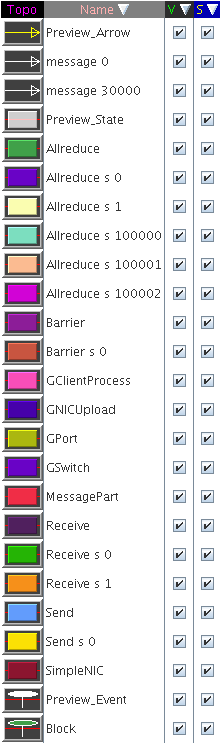
\includegraphics[scale=0.5]{Images/jumpshot-legend.png}
  }
\subfigure[Single iteration (with added states to define implementation)]{
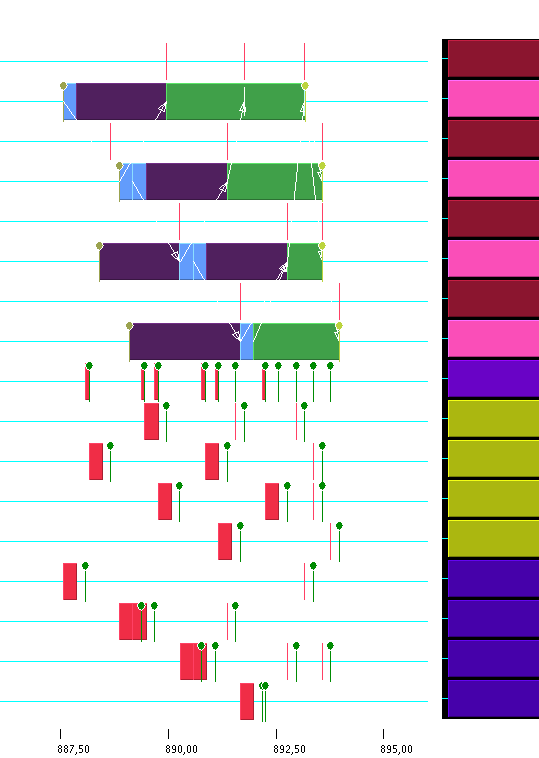
\includegraphics[scale=0.5]{Images/jumpshot-screenshot-1.png}
}

 \caption{Jumpshot screenshots for four clients}
   \label{fig:jumpshot_legend}
\end{figure}


\begin{figure}[!htbp]
  \centering
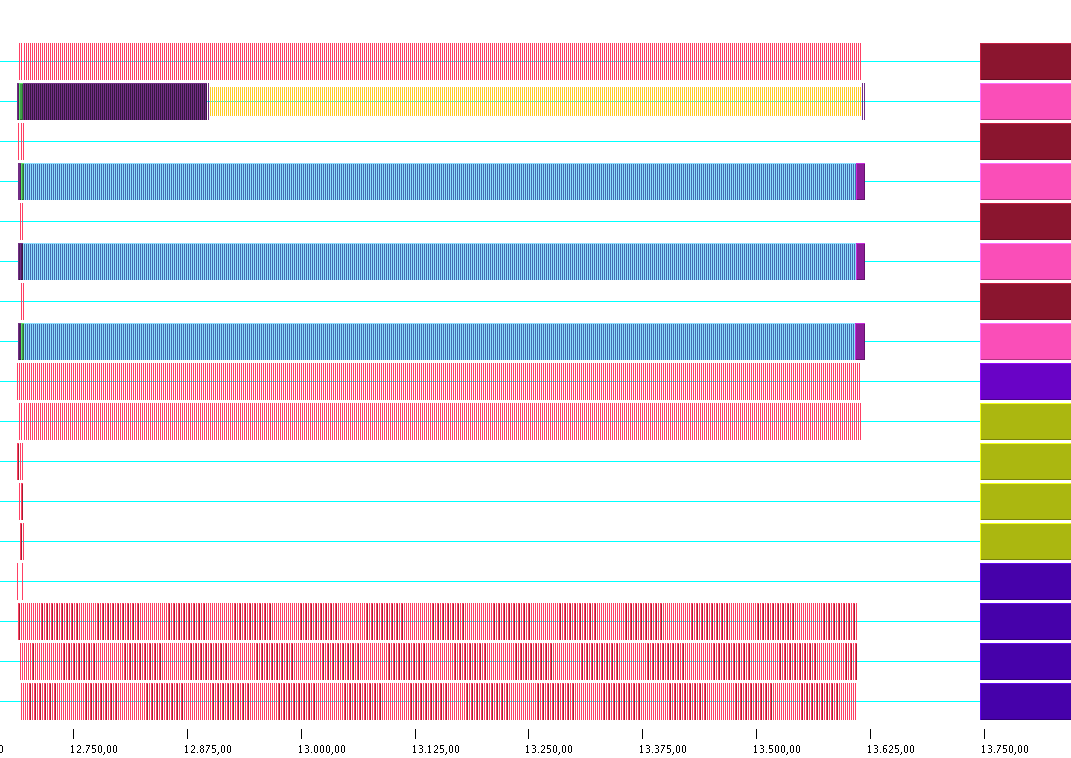
\includegraphics[scale=0.4]{Images/jumpshot-screenshot-2.png}
    \caption{Jumpshot screenshot of the final data collection and component markers}
    \label{fig:jumpshot_screenshot_2}
\end{figure}

\begin{table}
\begin{center}
\begin{tabular}{l||l|l|l}
Process count in \# & Real time in s & Simulated time in s & Simulated time / Real time \\
\hline
\hline
1 & 47.30 & 47.35 & 1.001 \\
2 & 24.79 & 24.93 & 1.006 \\
3 & 17.3 & 17.54 & 1.014 \\
4 & 13.54 & 13.75 & 1.016 \\
5 & 11.56 & 11.82 & 1.022 \\
6 & 10.09 & 10.33 & 1.024 \\
7 & 9.16 & 9.44 & 1.030 \\
8 & 8.39 & 8.73 & 1.041 \\
9 & 8.00 & 8.26 & 1.033
\end{tabular}
\end{center}
\caption{Comparison of simulation results with measured run time (rounded)}
\label{tbl:pde_results}
\end{table}


\subsection{Simulation speed}
* 100.000 events/second
* Simulation Speed, remove assertions 15 seconds vs. 3.5 seconds (debug/assertions) and 1.8 seconds with disabled debugging.

\subsection{Tracing}
Jumpshot
* Events which are traced: client activity (similar to the activity traced normally, with arrows to show message send/recv activity), different steps of the  commands, internal activity (network pakets)
* Example Images

\section{Code Documentation}
\subsection{JavaDoc}

\subsection{UML diagrams}
Done automatically via UMLGraph \footnote{\url{http://www.umlgraph.org/}}, JavaDoc annotations
allow to tune behavior.


\bibliographystyle{plainnat}
\bibliography{Bibliography}


\begin{appendix}
\chapter{Appendix}

\begin{lstlisting}[numbers=none,caption=Example code to build a disjoint client and server cluster model,label=lst:exampleClusterBuild,basicstyle=\ttfamily\scriptsize]
public ModelBuilder createDisjointClusterModel(int clients, int servers) throws Exception {

        int nodeCount = clients + servers;

        ModelBuilder mb = new ModelBuilder();

        // set global settings disjoint from default configuration:
        mb.getGlobalSettings().setTransferGranularity(100 * KBYTE);

        // build templates
        Connection conn = new Connection();
        conn.setName("1GBit Ethernet");
        conn.setLatency(new Epoch(0.0002));
        conn.setBandwidth(100 * MBYTE);
        mb.addTemplate(conn);

        Node node = new Node();
        node.setName("PVS-Node");
        node.setCPUs(1);
        node.setInstructionsPerSecond(1000000);
        node.setInternalDataTransferSpeed(1000 * MBYTE);
        node.setMemorySize(1000*1024*1024);

        NIC nic = new NIC();
        nic.setConnection(conn);

        mb.addNIC(node, nic);
        mb.addTemplate(node);

        RefinedDiskModel iosub = new RefinedDiskModel();
        iosub.setAverageSeekTime(new Epoch(0.005));
        iosub.setTrackToTrackSeekTime(new Epoch(0.001));
        iosub.setRPM(7200);
        iosub.setPositionDifferenceConsideredToBeClose(MBYTE * 5);
        iosub.setSequentialTransferRate(((int) 50 * MBYTE));
        iosub.setName("IBM");

        mb.addTemplate(iosub);

        SimpleSwitch sw = new SimpleSwitch();
        sw.setName("PVS-Switch");
        sw.setTotalBandwidth(380 * MBYTE);

        Port  port = new Port();
        port.setConnection(conn);
        for(int i=0; i <= nodeCount; i++)
                mb.addPort(sw, port);

        mb.addTemplate(sw);

        ///// NOW BUILD OBJECTS BASED ON PREVIOUS SETUP...

        SimpleSwitch testSW = mb.cloneFromTemplate(sw);
        ArrayList<Node> nodes = new ArrayList<Node>();

        mb.addSwitch(testSW);

        for (int i=0; i < nodeCount; i++){
                Node node2 = mb.cloneFromTemplate(node);
                nodes.add(node2);

                mb.addNode(node2);

                mb.setConnection(node2.getNICs().get(0), testSW.getPorts().get(i));
        }

        // example showing howto link two switches together:
        SimpleSwitch testSW2 = mb.cloneFromTemplate(sw);
        mb.addSwitch(testSW2);
        mb.setConnection(testSW.getPorts().get(nodeCount), testSW2.getPorts().get(nodeCount));

        for(int i=0; i < clients; i++ ){
                ClientProcess c = new ClientProcess();
                c.setName("Client" + i);
                mb.addClient(nodes.get(i), c);
                c.setRank(i);
                c.setApplication("Jacobi");
        }

        Server serverTemplate = new Server();
        serverTemplate.setName("Server");
        serverTemplate.setIOsubsystem(iosub);

        NoCache cacheImpl = new AggregationCache(); //NoCache()
        cacheImpl.setMaxNumberOfConcurrentIOOps(1);
        serverTemplate.setCacheImplementation(cacheImpl);

        mb.addTemplate(serverTemplate);

        for(int i=0; i < servers; i++ ){
                Server s = mb.cloneFromTemplate(serverTemplate);
                // disjoint client and server processes
                mb.addServer(nodes.get(i + clients), s);
        }

        //// Example howto change settings on all components using a particular template
        //conn.setName("10_GBit Ethernet");
        //conn.setLatency(new Epoch(0.00001));
        //conn.setBandwidth(1000 * MBYTE);
        //mb.modifyTemplateAndDerivedObjects("1GBit Ethernet", conn);

        return mb;
}
\end{lstlisting}

\listoffigures
\listoftables

\end{appendix}


\appendix


\end{document}
